\begin{figure}[H] \centering
\subsection{BDD (SK)}
{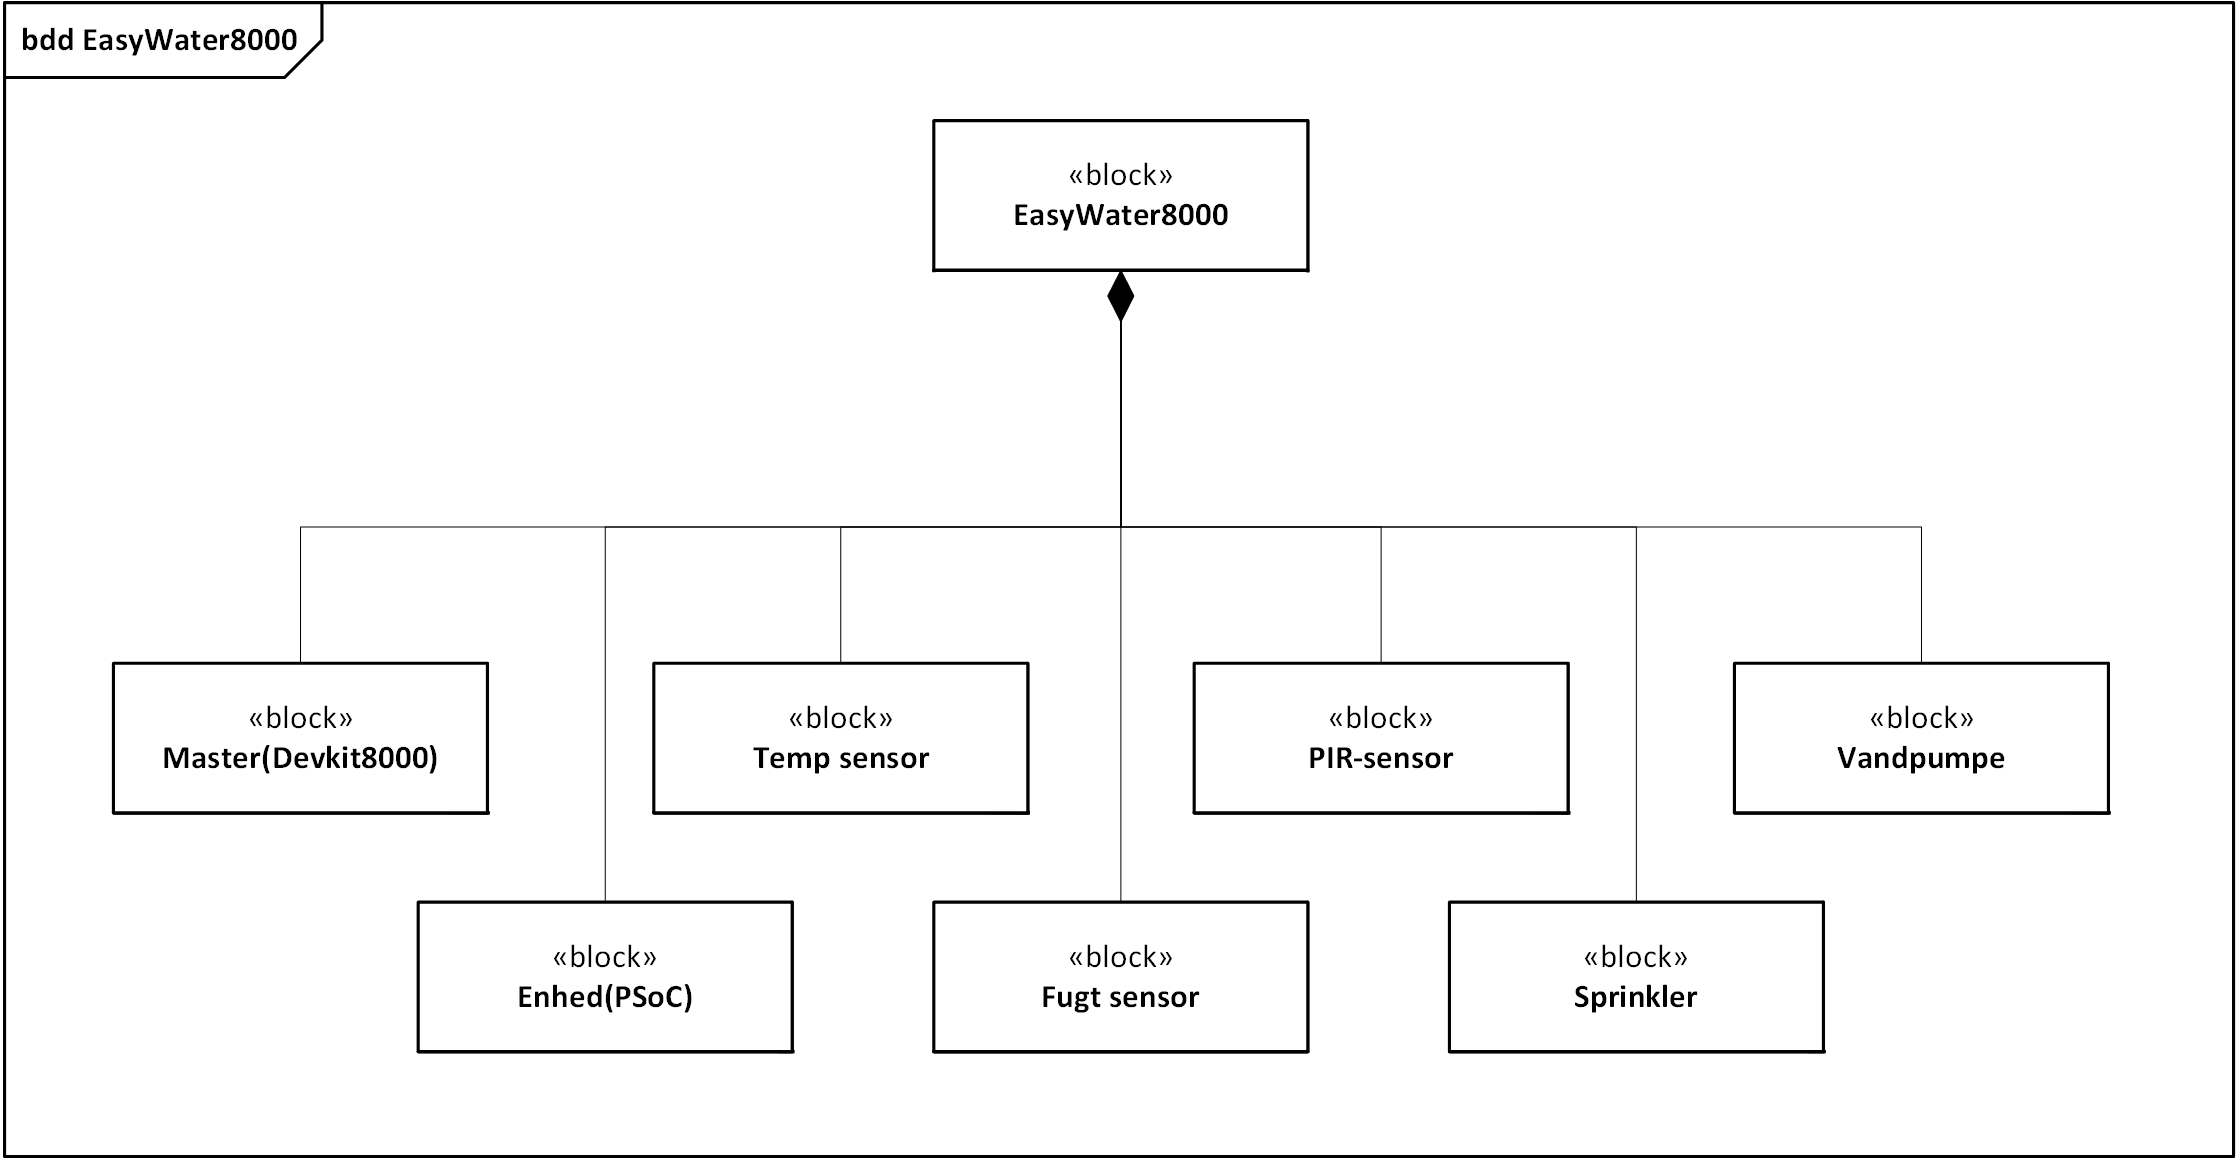
\includegraphics[width=0.9\textwidth]{filer/systemarkitektur/BDD}}
\caption{BDD}
\label{lab:bdd}
\raggedright
\end{figure}
BDD diagrammet giver et overblik over hvad det samlede system består af. Man ser en portbeskrivelse som viser hvilke signaler hver blok består af.

\begin{figure}[H] \centering
\subsection{BDD Master (MK)}
{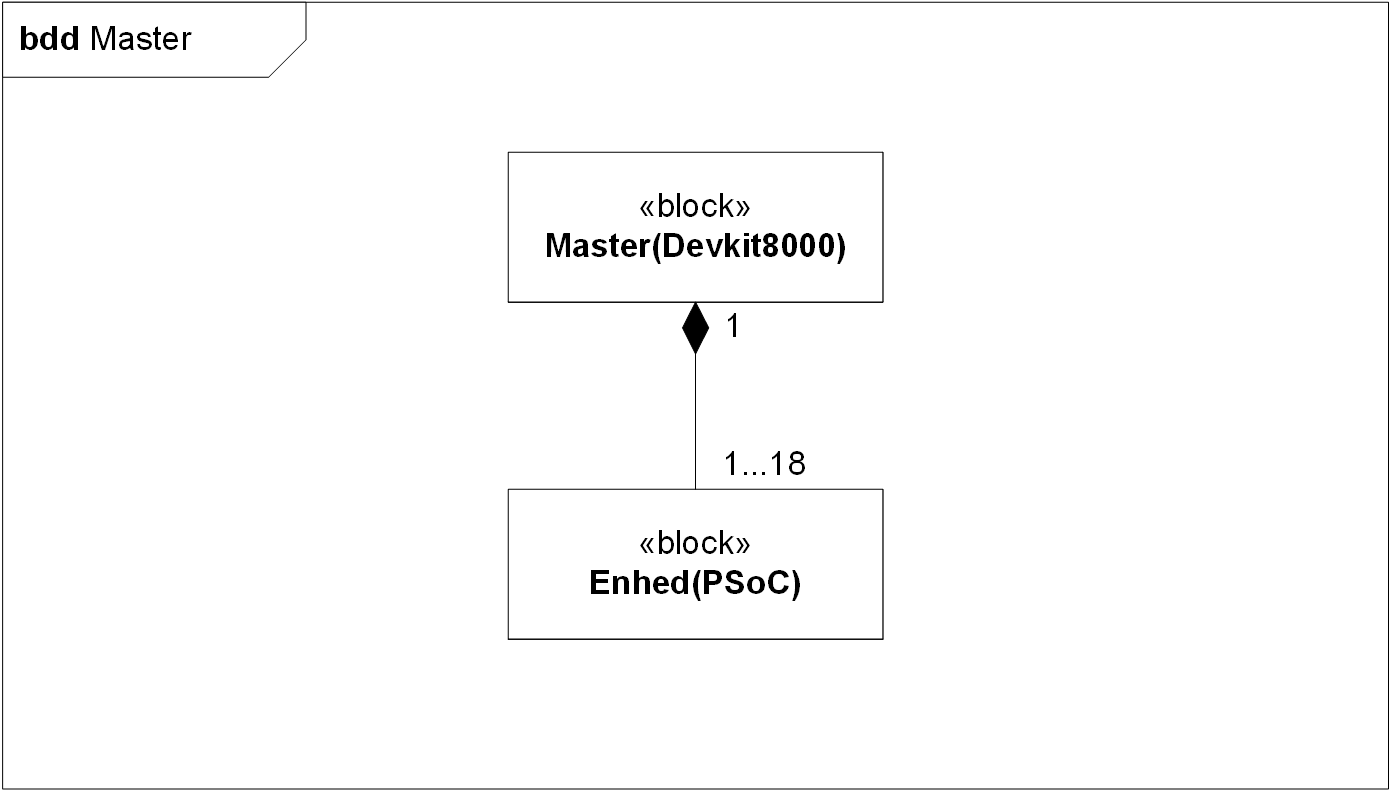
\includegraphics[width=0.9\textwidth]{filer/systemarkitektur/BDD_Master}}
\caption{BDD Master}
\label{lab:bddmaster}
\raggedright
\end{figure}
BDD diagrammet giver et overblik over hvad Master består af.

\begin{figure}[H] \centering
\subsection{BDD Enhed (MK)}
{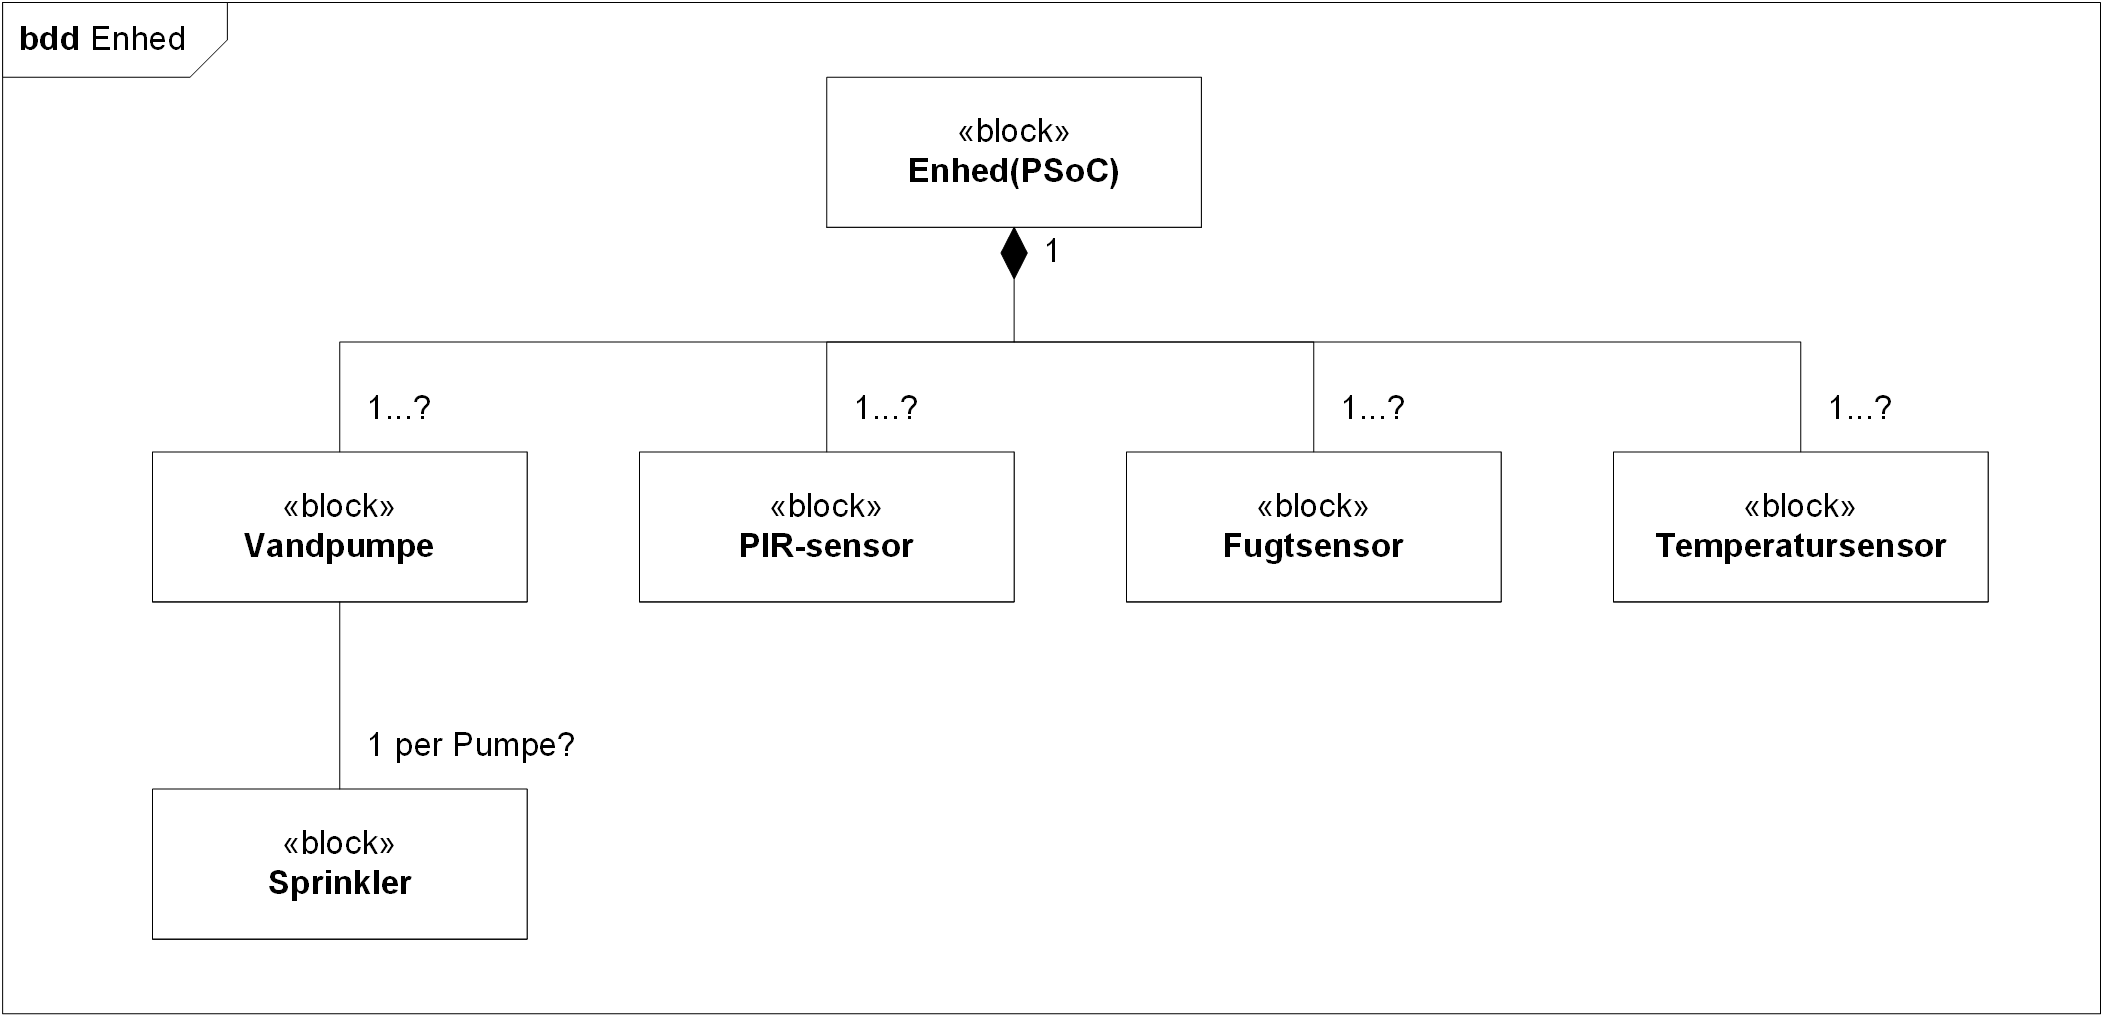
\includegraphics[width=0.9\textwidth]{filer/systemarkitektur/BDD_Enhed}}
\caption{BDD Enhed}
\label{lab:bddenhed}
\raggedright
\end{figure}
BDD diagrammet giver et overblik over hvad Enhed består af.

\begin{figure}[H] \centering
\subsection{IBD (SK)}
{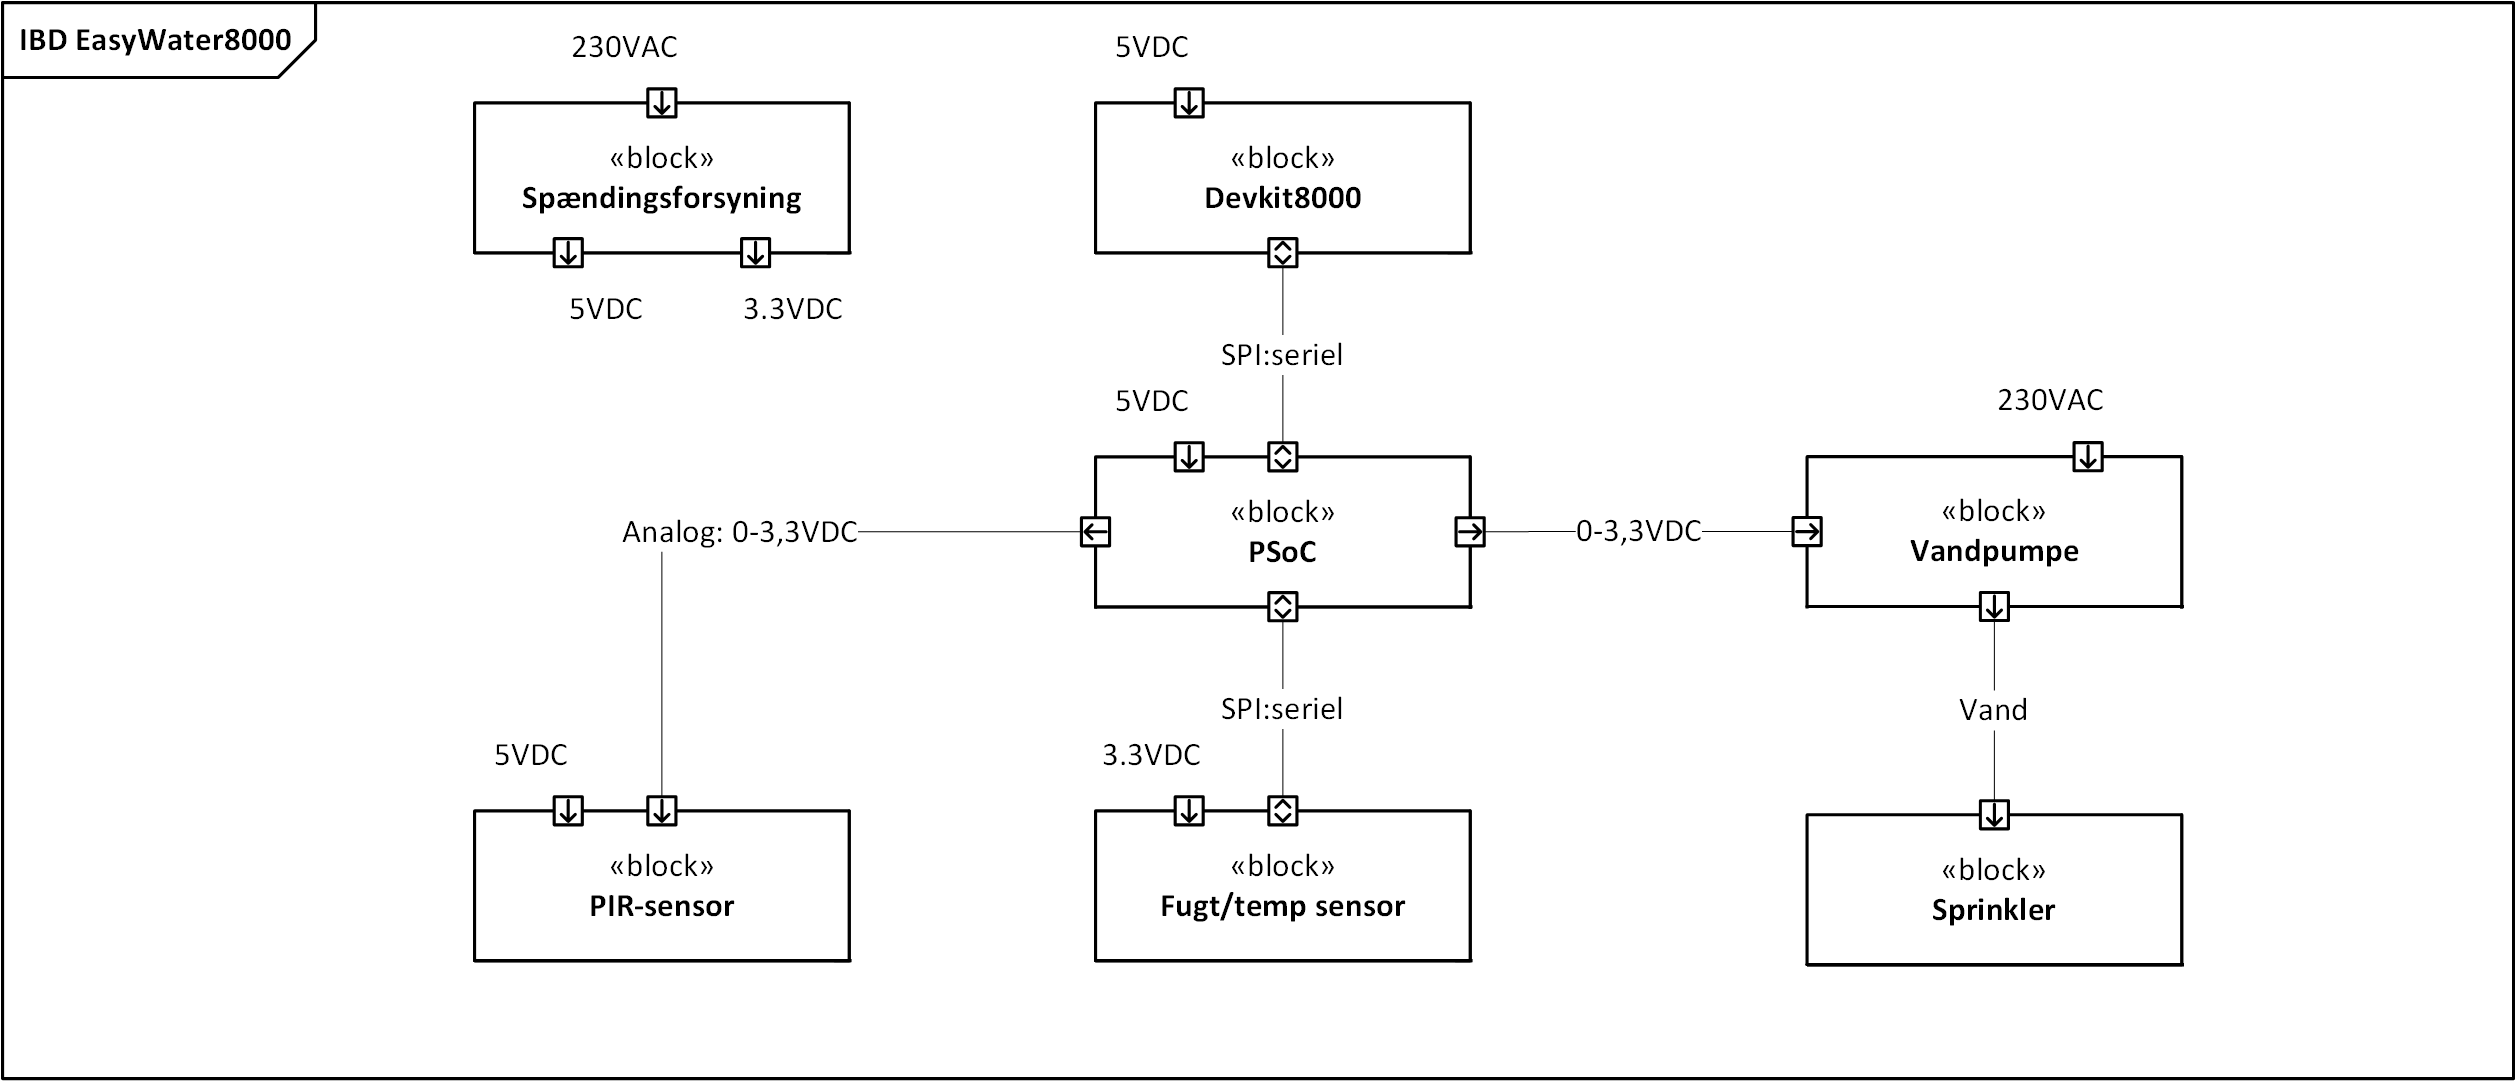
\includegraphics[width=0.9\textwidth]{filer/systemarkitektur/IBD}}
\caption{IBD}
\label{lab:ibd}
\raggedright
\end{figure}
IBD diagrammet giver et internt overblik over hvordan hele vores system er forbundet. Vi ser hvilke type signaler der bliver sendt imellem de forskellige blokke.
